\documentclass{praktikum}
\usepackage{graphicx}
\usepackage{caption}
\usepackage{subcaption}
\graphicspath{ {./} }
\usepackage{pgfplotstable}
%====== Vyplňte údaje ======
%% dobrá rada na začátek - pokud nevíš, co měníš, zálohuj to, co funguje ;)

\jmeno{Matyáš Peroutík}
\kod{256371}
\rocnik{1}
\obor{AMT}
\skupina{}
\labskup{B}
\spolupracoval{Štěpán Pavlica}


\ucitel{}
\merenodne{27.\,03.\,2024}
\odevzdanodne{03.\,04.\,2024}

\priprava{}
\opravy{}
\nazev{Hallův Jev}
\cislo{27} %měřené úlohy

\usepackage{fancyhdr}
\usepackage{lastpage}
\pagestyle{fancy}
\fancyhf{}
\renewcommand{\headrulewidth}{0pt}
 
\rfoot{Strana \thepage \hspace{1pt} z \pageref{LastPage}}

\begin{document}

%====== Vygenerování tabulky ======
\maketitle
\vspace{0.5 cm}

%====== Text protokolu zde ======

\section{Úkol měření}
\begin{enumerate}
\item Změřte závislost Hallova napětí na proudu vzorkem pro oba směry proudu a oba směry magnetické indukce.
\item Určete velikost Hallovy konstanty vzorku.
\item Určete, o kolik koncentrace majoritních nosičů náboje převyšuje koncentraci nosičů minoritních
\item Proměřte závislost velikosti Hallova napětí na velikosti indukce magnetického pole.
\end{enumerate}
\section{Teoretický rozbor}

\subsection{Hallův jev}
V této sekci budeme uvažovat za vzorek tenkou měděnou destičku nebo plech o šířce b a tloušťce c a elektrickým proudem tekoucím ve směru naznačeném na \textit{Obrázku~\ref{img:hall_kovy}a}.

\begin{figure}[H]

\centering
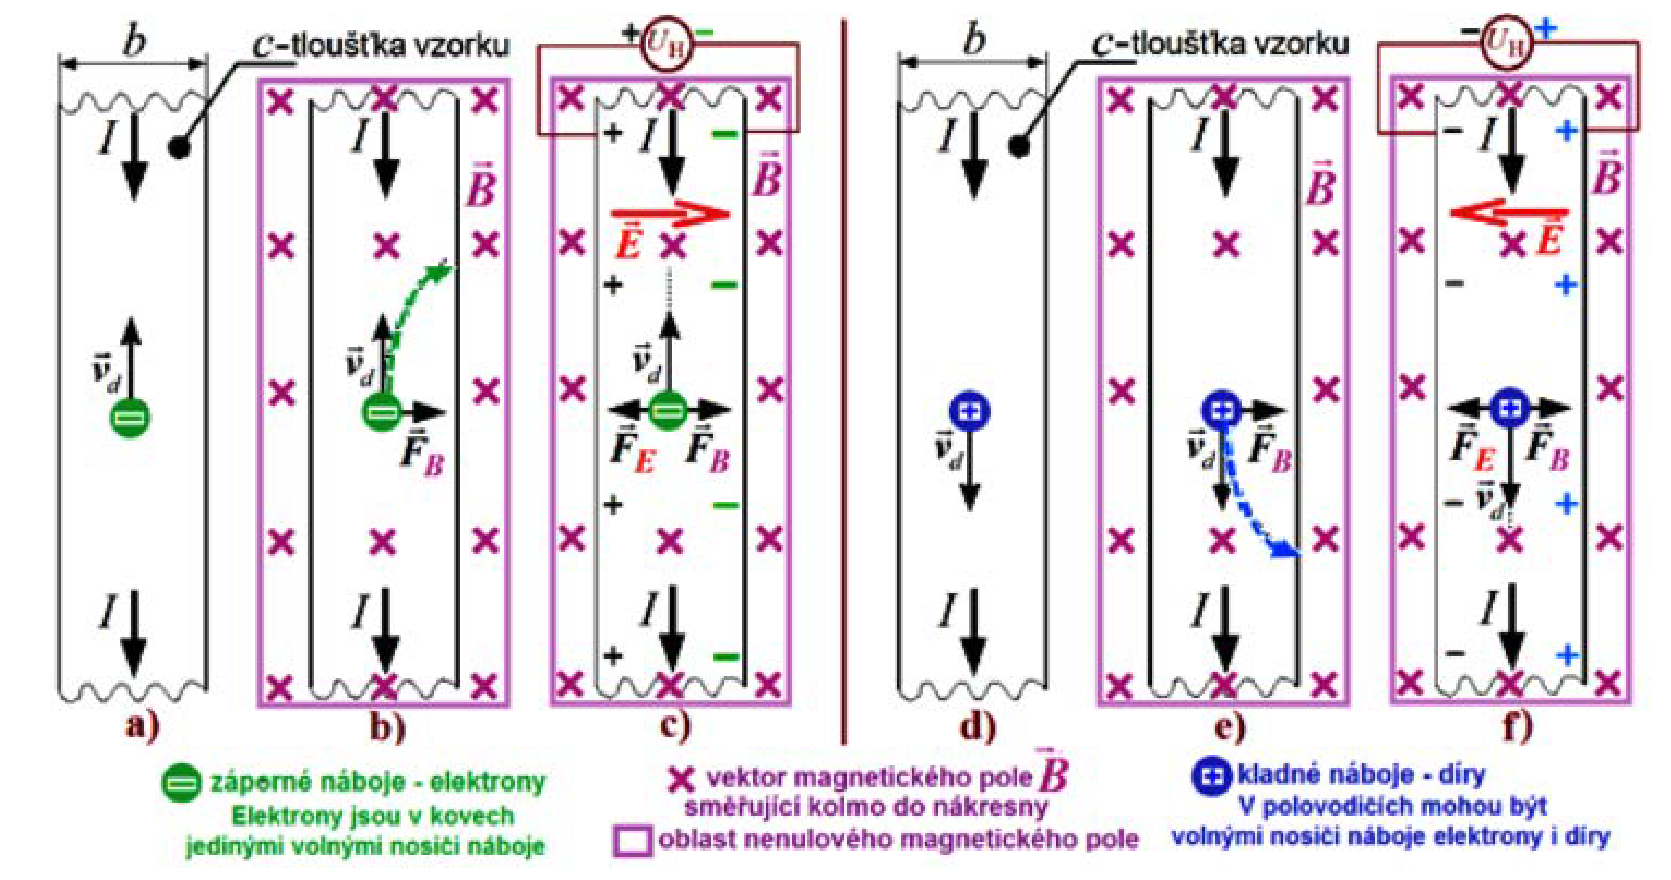
\includegraphics[width=0.82\textwidth]{hall_kovy}
\caption{Hallův jev v kovovém vzorku}\label{img:hall_kovy}
\end{figure}
\paragraph{}
Díky tomuto proudu se elektrony pohybují driftovou rychlostí $\overrightarrow{v_d}$. Pokud vzorek vložíme do magnetického pole, začne na elektrony působit Lorentzova síla, která lze spočítat pomocí vztahu:

\begin{equation}
\label{eqn:theory_fb_lorenz_force}
\overrightarrow{F_B} = q\overrightarrow{v_d}\times \overrightarrow{B}
\end{equation}
$\overrightarrow{F_B}$ \dotfill Vektor Lorentzovy síly \linebreak
q \dotfill Náboj částice, na kterou síla působí \linebreak
$\overrightarrow{v_d}$ \dotfill Vektor driftové rychlosti částice \linebreak
$\overrightarrow{B}$ \dotfill Vektor magnetické indukce \linebreak

Kvůli tomuto se začnou elektrony kupit na jedné straně vzorku (za předpokladu směrů mag. indukce viz. Obrázek~\ref{img:hall_kovy}b), což způsobí vznik elektrického pole, které bude další příchozí elektrony odpuzovat silou s opačným směrem, než měla síla $\overrightarrow{F_B}$. (viz. Obrázek~\ref{img:hall_kovy}b). Velikost této síly je dána následujícím vztahem:

\begin{equation}
\label{eqn:theory_fe_electrical_force}
\overrightarrow{F_E} = q\overrightarrow{E}
\end{equation}
$\overrightarrow{F_E}$ \dotfill Vektor síly způsobené působením el. pole na částici \linebreak
q \dotfill Náboj částice, na kterou síla působí \linebreak
$\overrightarrow{E}$ \dotfill Vektor elektrického pole \linebreak

Po uplynutí krátkého časového okamžiku se tyto dvě síly navzájem vyruší a začnou se opět pohybovat ve svém původním směru (viz. Obrázek~\ref{img:hall_kovy}c). Oproti původnímu stavu zde přibylo elektrické pole $\overrightarrow{E}$, jehož následek je vznik napětí mezi dvěmi stranami vzorku. Toto napětí nazýváme Hallovo napětí a značíme ho $U_H$. Pro polovodiče platí stejné zákonitosti pro záporné náboje. \hfill \\
 \indent Opačně působí tyto síly i na kladné nosiče nábojů (viz. Obrázek~\ref{img:hall_kovy}d,e,f). Pokud by bylo ve vzorku shodné množství kladných a záporných nábojů, tak by navzájem vykompenzovali elektrické pole a Hallovo napětí by bylo nulové. S tímto jevem ee můžeme setkat ve vlastních polovodíčích. U polovodičů typu N převažují záporné náboje a u polovodičů typu P převažují kladné náboje. Tudíž u nich hallovo napětí naměříme. U izolantů nejsou téměř žádné volné nosiče, a tudíž zde hallovo napětí také nenaměříme.
 
\subsection{Princip metody měření}
Jednoduchým odvozením z rovnováhy sil lze získat u kovů vztah pro výpočet Hallova napětí:
\begin{equation}
\label{eqn:theory_uh_odvozene}
U_H = \frac{1}{nq}\frac{BI}{c}
\end{equation}
n \dotfill Koncentrace volných nosičů náboje \linebreak
q \dotfill Velikost náboje nosiče \linebreak
B \dotfill Velikost magnetické indukce \linebreak
I \dotfill Velikost proudu protékající vzorkem \linebreak
c \dotfill Tloušťka vzorku \newpage 

Zlomek bez veličin B, I, c je označován jako Hallova konstanta, která je označována $R_H$. Pro kovy platí nasledující vztah:

\begin{equation}
\label{eqn:theory_rh_hall_kovy}
R_H = \frac{1}{nq}
\end{equation}

pro polovodiče:
\begin{equation}
\label{eqn:theory_rh_hall_polovodiče}
R_H = \frac{3\pi}{8}\frac{1}{nq}
\end{equation}

Po dosazení konstanty do vztahu můžeme vidět, že závislost je přímo úměrná jak magnetické indukci, tak i procházejícímu proudu. Díy tomu, že je jednodušší nastavovat proud, budeme při měření ponechávat magnetickou indukci konstantní.

\begin{equation}
\label{eqn:theory_uh_lin}
U_H = R_H\frac{B}{c}I = kI
\end{equation}

Jelikož se jedná o lineární závislost a všechny veličiny až na směrnici k jsou konstanty, můžeme pomocí ní stanovit Hallovu konstantu

\begin{equation}
\label{theory_k_rh_hallovka}
k = R_H\frac{B}{c} \quad \quad
R_H = \frac{kc}{B}
\end{equation}

Pokud bude proud tvořen hlavně kladnými náboji, vyjde Hallova konstanta > 0, pokud zápornými náboji tak < 0.

\section{Schéma zapojení}
\begin{figure}[H]
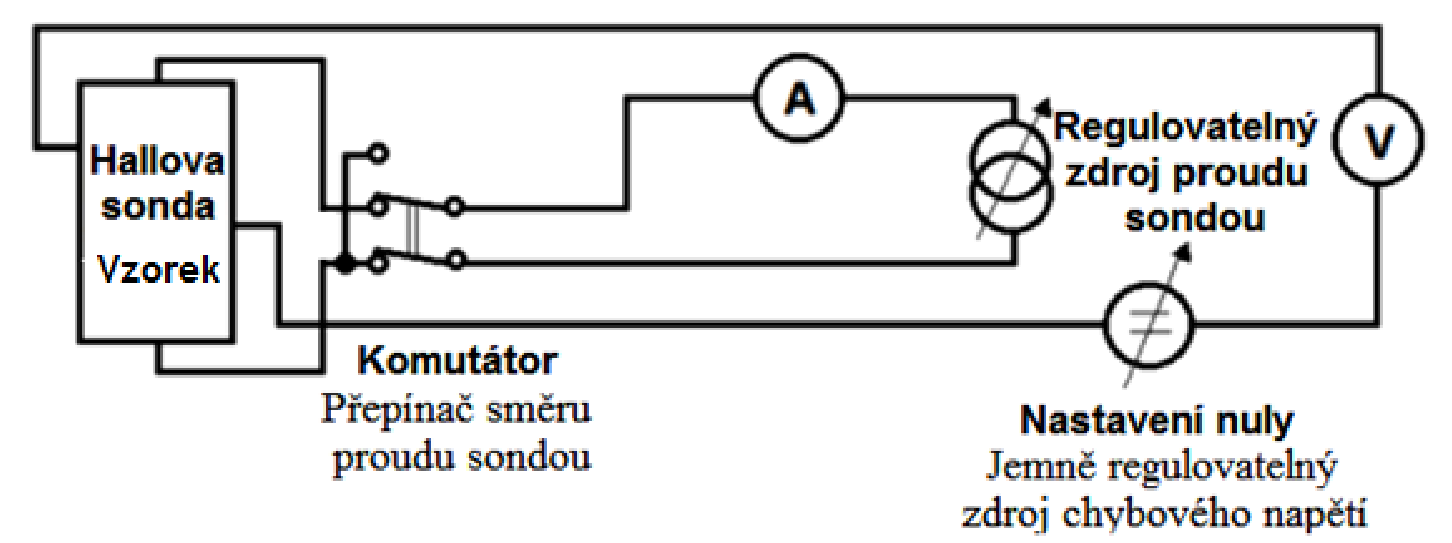
\includegraphics[width=\textwidth]{schena}
\label{img:schema}
\caption{Obvodové schéma aparatury s hallovou sondou}
\end{figure}

\newpage

\section{Naměřené hodnoty}

\begin{table}[H]
\begin{adjustbox}{width=\columnwidth,center}
    %\centering
    \renewcommand{\arraystretch}{1.5}
    \pgfplotstabletypeset[
    columns/0/.style={column name={č}},
    columns/1/.style={column name={$ \dfrac{I}{[mA]}$}},
    columns/2/.style={column name={$\dfrac{U_{H1}}{[mV]}$}},
    columns/3/.style={column name={$\dfrac{U_{H2}}{[mV]}$}},
    columns/4/.style={column name={$\dfrac{U_{H3}}{[mV]}$}},
    columns/5/.style={column name={$\dfrac{U_{H4}}{[mV]}$}},
    skip first n={1},
    header=false,
    string type,
    before row=\hline,
    every last row/.style={after row=\hline},
    column type/.add={|}{},
    every last column/.style={column type/.add={}{|}},
    every head row/.style={
    before row={\multicolumn{6}{c}{Tloušťka Hallova vzorku c = 0,6 mm} \\
        \hline
         \multicolumn{2}{|c|}{}  & \multicolumn{4}{|c|}{Kombinace} \\
         \hline
        \multicolumn{2}{|c|}{} & A-0 & A-180 & B-0 & B-180 \\
        \hline
         \multicolumn{2}{|c|}{Komutátor} & Nahoře A & Nahoře A & Dole B & Dole B\\
         \hline
         \multicolumn{2}{|c|}{úhel} & 0° & 180° & 0° & 180° \\ 
         \hline},
    },
]{kombinace.dat}%

    \hspace{0,5cm}
    \renewcommand{\arraystretch}{1.2}
    \pgfplotstabletypeset[
    columns/0/.style={column name={$\dfrac{\text{úhel}}{[\text{°}]}$}},
    columns/1/.style={column name={$\dfrac{B}{[mT]}$}},
    columns/2/.style={column name={$\dfrac{U_H}{[mV]}$}},
    columns/3/.style={column name={$\dfrac{\text{úhel}}{[\text{°}]}$}},
    columns/4/.style={column name={$\dfrac{B}{[mT]}$}},
    columns/5/.style={column name={$\dfrac{U_H}{[mV]}$}},
    skip first n={1},
    header=false,
    string type,
    before row=\hline,
    every last row/.style={after row=\hline},
    column type/.add={|}{},
    every last column/.style={column type/.add={}{|}},
    every head row/.style={
    before row={\multicolumn{6}{c}{Měřeno pro I = 2,2 mA} \\
        \hline},
    },
]{intenzity.dat}%
    %\caption{Caption}
    \label{tab:my_label}
\end{adjustbox}
\end{table}

\section{Zpracování hodnot}
Grafy závislosti Hallova napětí na protékajícím proudu při indukci 70mT
\begin{figure}[H]
\centering
\hspace*{-1.5cm}

\begin{minipage}{.5\textwidth}\hspace*{-1.5cm}
  \centering
  \begin{tikzpicture}
\begin{axis}[
    legend entries={$U_{H1}$,{$k_1 = 50.46VA^{-1}$}},
legend style={at={(0.5,1.15)},anchor=north, legend columns=-1},
xlabel=$ \dfrac{I}{[mA]}$,
ylabel=$\dfrac{U_{H}}{[mV]}$]
\addplot + table[only marks, x={I}, y={U1}, /pgf/number format/read comma as period] {kombAbs.dat};
\addplot + table[mark=none, x={I}, y={U1}, /pgf/number format/read comma as period] {kombAbs.dat};
\end{axis}
\label{grf:u1(i)}
\end{tikzpicture}
  \captionof{figure}{Komutátor nahoře, úhel $0$}
\end{minipage}%
\begin{minipage}{.5\textwidth}\hspace*{-0.5cm}
  \centering
  \begin{tikzpicture}
\begin{axis}[
    legend entries={$U_{H2}$,{$k_2 = 50.93VA^{-1}$}},
legend style={at={(0.5,1.15)},anchor=north, legend columns=-1},
xlabel=$ \dfrac{I}{[mA]}$,
ylabel=$\dfrac{U_{H}}{[mV]}$]
\addplot + table[only marks, x={I}, y={U2}, /pgf/number format/read comma as period] {kombAbs.dat};
\addplot + table[mark=none, x={I}, y={U2}, /pgf/number format/read comma as period] {kombAbs.dat};
\end{axis}
\label{grf:u2(i)}
\end{tikzpicture}
  \captionof{figure}{Komutátor nahoře, úhel $180$}
  
\end{minipage}
\end{figure}


\begin{figure}[H]
\centering


\begin{minipage}{.5\textwidth}\hspace*{-1.5cm}
  \centering
  \begin{tikzpicture}
\begin{axis}[
legend entries={$U_{H3}$,{$k_3 = 50.35VA^{-1}$}},
legend style={at={(0.5,1.15)},anchor=north, legend columns=-1},
xlabel=$ \dfrac{I}{[mA]}$,
ylabel=$\dfrac{U_{H}}{[mV]}$]
\addplot + table[only marks, x={I}, y={U3}, /pgf/number format/read comma as period] {kombAbs.dat};
\addplot + table[mark=none, x={I}, y={U3}, /pgf/number format/read comma as period] {kombAbs.dat};
\end{axis}
\label{grf:u3(i)}
\end{tikzpicture}
  \captionof{figure}{Komutátor dole, úhel $0$}
\end{minipage}%
\begin{minipage}{.5\textwidth}\hspace*{-0.5cm}
  \centering
  \begin{tikzpicture}
\begin{axis}[
    legend entries={$U_{H4}$,{$k_4 = 50.94VA^{-1}$}},
legend style={at={(0.5,1.15)},anchor=north, legend columns=-1},
xlabel=$ \dfrac{I}{[mA]}$,
ylabel=$\dfrac{U_{H}}{[mV]}$]
\addplot + table[only marks, x={I}, y={U4}, /pgf/number format/read comma as period] {kombAbs.dat};
\addplot + table[mark=none, x={I}, y={U4}, /pgf/number format/read comma as period] {kombAbs.dat};
\end{axis}
\label{grf:u4(i)}
\end{tikzpicture}
  \captionof{figure}{Komutátor dole, úhel $180$}
  
\end{minipage}
\end{figure}

Z těchto grafů jsme regresí získali 4 směrnice k, ze kterých se dá vyvést její průměrná hodnota pomocí studentova rozložení.

\[ \overline{k} = \frac{\sum k_i}{n} \doteq 50.67 VA^{-1} \]
\[ s^2 = \frac{\sum (\overline{k}-k_i)^2}{n-1} \doteq 0.9567 V^2A^{-2}\]
\[ s = \sqrt{\frac{\sum (\overline{k}-k_i)^2}{n-1}} \doteq 0.3093VA^{-1} \]
\[ \delta (k) = t_{4;0.95} \cdot \frac{s}{\sqrt{n}} \doteq 0.5091 VA^{-1} \]
\[ \delta_r (k) = \frac{\delta (k)}{\overline{k}} \doteq 0.01005 \]
\[ k = (50.7 \pm 0.5) VA^{-1} \]

Následně se dá pomocí vztahu (\ref{theory_k_rh_hallovka}) spočítat Hallova konstanta:

\[ \overline{R_H} = \overline{k}\frac{\overline{c}}{\overline{B}} \doteq 0.4343 m^3C^{-1} \]

A následně také chyba výpočtu Hallovy konstanty:
\[ \delta (R_H) = 
\sqrt{\left( \frac{\partial R_H}{\partial k}\delta(k) \right) ^2 +
\left( \frac{\partial R_H}{\partial c}\delta(c) \right) ^2 +
\left( \frac{\partial R_H}{\partial B}\delta(B) \right) ^2
} \doteq 0.03645 m^3C^{-1}  \]
\[ \delta_r (R_H) = \frac{\delta (R_H)}{\overline{R_H}} \doteq 0.08394 \]

Poté můžeme odvodit skutečnou velikost Hallovy konstanty:
\[R_H = (0.43 \pm 0.04) m^3C^{-1} \]

Dále můžeme pomocí vztahu (\ref{eqn:theory_rh_hall_polovodiče}) určit, o kolik převyšuje koncentrace majoritních nosičů koncentraci nosičů minoritních.

\[ n = \frac{3 \pi}{8} \frac{1}{R_Hq} \doteq 1.69 \cdot 10 ^ {19} m ^ {-3}\]

Relativní chyba bude stejná jako byla u Hallovy konstanty. Poté výsledná koncentrace bude:
\[ n = ( 1.69\pm 0.14) \cdot 10 ^ {19} m ^ {-3}\]

\subsection{Legenda k výpočtům}

$\overline{k}$ \dotfill Průměrná hodnota směrnic grafů \\
$s^2$ \dotfill Rozptyl směrnic grafů \\
s \dotfill Směrodatná odchylka směrnic grafů \\
$\delta (k)$ \dotfill Absolutní chyba směrnice grafů \\
$\delta_r (k)$ \dotfill Relativní chyba směrnice grafů \\
k \dotfill Hodnota směrnice grafů \\
$\overline{R_H}$ \dotfill Průměrná hodnota Hallovy konstanty \\
$\delta (R_H)$ \dotfill Absolutní chyba Hallovy konstanty \\
$\delta_r (R_H)$ \dotfill Relativní chyba Hallovy konstanty \\
$R_H$ \dotfill Velikost Hallovy konstanty \\
$t_{4;0.95}$ \dotfill Koeficient Studentova rozložení 3.292 \\
$\delta_r(c)$ \dotfill Relativní chyba tloušťky vzorku \\
$\delta_r(B)$ \dotfill Relativní chyba kalibrovaného mag. toku \\
q \dotfill Náboj jednoho elektronu $1.602\cdot 10^{-19}C$ \\
n \dotfill Koncentrace mjoritních nábojů \\

\subsection{Závislost Hallova napětí na mag. indukci při konst. proudu 2.2mA}

\begin{tikzpicture}
\begin{axis}[
width=15cm,
height = 8cm,
xlabel=$ \dfrac{I}{[mA]}$,
ylabel=$\dfrac{U_{H}}{[mV]}$]
\addplot table[x={b1}, y={u1}, /pgf/number format/read comma as period] {intenzity.dat};
\addplot table[x={b2}, y={u2}, /pgf/number format/read comma as period, scatter] {intenzity.dat};
\end{axis}
\end{tikzpicture}

\section{Závěr}
\paragraph{}
Při tomto měření jsme zjistili hodnotu Hallovy konstanty vzorku $R_H = (0.43 \pm 0.04) m^3C^{-1}$. Dále jsme naměřili, že koncentrace majoritních nosičů (elektronů) převyšuje koncentraci minoritních nosičů (děr) o $n = ( 1.69\pm 0.14) \cdot 10 ^ {19} m ^ {-3}$. Z grafu závislosti Hallova napětí na magnetické indukci při konstantním proudu 2.2mA můžeme sledovat, že závislost je téměř lineární. \\
\indent Chyby měření pravděpodobně vznikly teplotní bilancí, nebo možným pootočením ukazatele aktuálního úhlu pootočení. Dalším zdrojem chyby mohly být vysoké tolerance součástek, nebo nepřesností hodnot v kalibrační tabulce. Nejvyšší chyby se objevovali u závislosti Hallova napětí na mag. indukci poblíž nulové mangetické indukce.
\end{document}

